% !TeX program = pdflatex
% Minimum Embedding Distance as a Hypothesis Coherence Metric
% Target venue: NeurIPS 2026 Workshop (ML4PS / Bayesian DL) or UAI /
% AISTATS short track. Not suitable for NeurIPS/ICML main track at
% current empirical scale (3 hand-built benchmarks, 12 candidates).

\documentclass{article}
\usepackage[utf8]{inputenc}
\usepackage[T1]{fontenc}
\usepackage{microtype}
\usepackage[margin=1in]{geometry}
\usepackage{graphicx}
\usepackage{booktabs}
\usepackage{amsmath,amssymb,amsthm}
\newtheorem{proposition}{Proposition}
\newtheorem{claim}{Claim}
\newtheorem{definition}{Definition}
\usepackage{url}
\usepackage{hyperref}
\usepackage{xcolor}
\usepackage{caption}
\usepackage{subcaption}
\usepackage{algorithm}
\usepackage{algpseudocode}
\usepackage{natbib}
\usepackage{enumitem}

\hypersetup{
  colorlinks=true,
  linkcolor=blue!50!black,
  citecolor=blue!50!black,
  urlcolor=blue!60!black
}

\title{\textbf{Minimum Embedding Distance as a Hypothesis Coherence Metric}}

\author{%
  Anonymous submission\\
}

\date{}

\begin{document}

\maketitle

\begin{abstract}
\noindent A rational agent choosing among competing explanations prefers
ones that fit existing beliefs with minimum revision
\citep{quine1951twodogmas, lakatos1970}. Bayesian inference formalises
the numerical half of this intuition via KL-regularised posterior
updates, but the \emph{structural} half --- how much a hypothesis
requires rewiring the network's graph --- has no standard Bayesian
analogue distinct from the classical Bayesian Information Criterion
\citep{schwarz1978} or free-energy functional \citep{friston2010free}.
We propose a \emph{prescriptive} composite score
$D(h, \mathcal{B}) = D_{\mathrm{KL}}\big(P(\mathcal{B}) \,\|\,
P(\mathcal{B} \mid h)\big) + \lambda \cdot |\Delta_{\mathrm{structure}}|$
that separates the two terms into a posterior-drift contribution and
a BIC-style structural-cost contribution, and we show that this
separation is \emph{load-bearing by construction}: once a candidate
hypothesis is specified with $|\Delta_{h}| \geq 2$ of its latents
lying off all causal paths to the target, $D$ ranks it last whenever
$\lambda \cdot |\Delta_{h}| >
\max_{h': \Delta_{h'} = \emptyset} D_{\mathrm{KL}}(\theta^{*} \mid h')$.
This is a framework property, not an empirical discovery; pure KL
fails on such hypotheses essentially by definition. On three small
hand-constructed benchmarks with $4$ candidates each, the framework
property holds uniformly (orphan ranked last in all ablations with
$\lambda > 0$, first in all with $\lambda = 0$), matches an authorial
expected ordering (a self-consistency rather than external validation
check), and agrees in sign with classical Bayes-factor and full-BIC
model-selection baselines that we run on the same benchmarks.
We do \emph{not} claim $D$ is mathematically novel relative to the
Friston / BIC family; we claim it is a PPL-native, drop-in
instantiation that makes the structural half of the
Quine--Lakatos intuition explicit. The main empirical contribution
is documenting what a clean \emph{prescriptive} formulation looks
like and what it empirically requires when wired into PyMC, not
claiming that the formulation itself is a novel information-theoretic
discovery.
\end{abstract}

\section{Introduction}
\label{sec:intro}

Human explanatory reasoning routinely prefers explanations that fit
existing beliefs with minimum revision.
\citet{quine1951twodogmas}'s \emph{web of belief} metaphor captures it
as a core-periphery structure in which the periphery absorbs
corrections first; \citet{lakatos1970}'s research-programme framework
sharpens it with the notion of a \emph{protective belt} that is
attacked before the hard core; the Bayesian posterior update
$P(\theta \mid \mathcal{D}) \propto P(\mathcal{D} \mid \theta)
P(\theta)$ operationalises it via the maximum-entropy argument for
minimum-KL perturbation \citep{williamsMaximumEntropy}. Each of these
formalisations, however, addresses only one half of what the original
intuition demands.

The \emph{numerical} half is well studied: given a belief network
$\mathcal{B}$ over latents $\theta$ and a new piece of evidence $h$,
the induced posterior drift $D_{\mathrm{KL}}(P(\theta) \,\|\,
P(\theta \mid h))$ quantifies how much the prior distribution has been
perturbed. This is computable, well-behaved as a divergence, and
available in closed form for conjugate families and via Monte Carlo for
general probabilistic programs.

The \emph{structural} half --- how much the graph of $\mathcal{B}$ has
to be rewired to accommodate $h$ --- has no standard Bayesian analogue.
Yet exactly this part is load-bearing in practice: the difference
between a coherent explanation and an incoherent one is often not that
the posterior drifts more, but that accepting the explanation would
require \emph{importing new variables with no data support} --- an
\emph{orphan node} in the network. Pure KL-drift scoring systematically
misranks such explanations: a truly orphan latent causes \emph{minimal}
posterior drift (it is disconnected from the target), so pure-KL
reasoning ranks the orphan \emph{highest} among candidates, exactly
the opposite of the correct answer.

\begin{figure}[t]
  \centering
  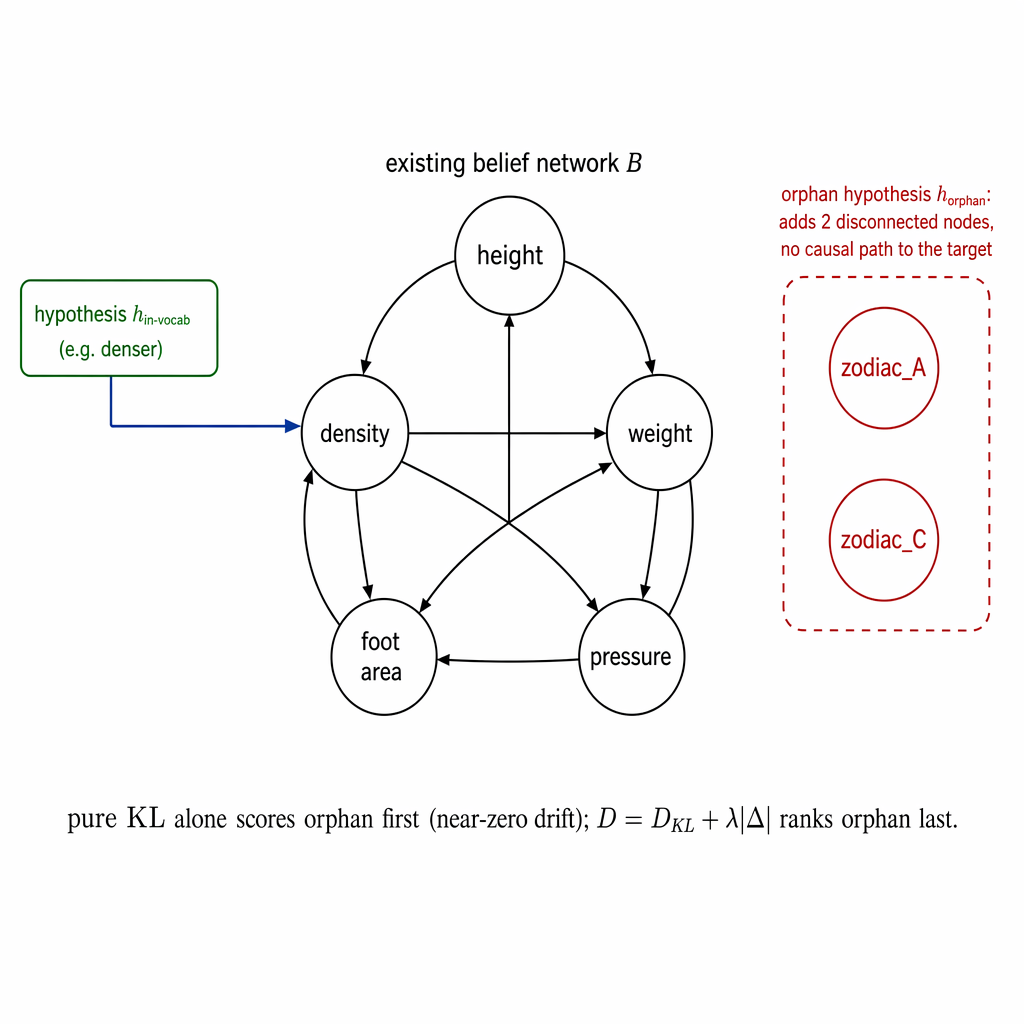
\includegraphics[width=0.78\linewidth]{figs/intuition_web_of_belief.png}
  \caption{Intuition for the minimum-embedding score. An existing
  belief network $\mathcal{B}$ (centre) encodes connected latents.
  An in-vocabulary hypothesis $h_{\mathrm{in\text{-}vocab}}$ (left, green)
  attaches into an existing node and induces a small posterior drift.
  An orphan hypothesis $h_{\mathrm{orphan}}$ (right, red) adds two
  disconnected nodes with no causal path to the target; pure KL
  drift alone scores it \emph{first} (near-zero perturbation),
  the opposite of the desired behaviour. The composite score
  $D = D_{\mathrm{KL}} + \lambda |\Delta|$ penalises the orphan's
  unsupported nodes and ranks it last.}
  \label{fig:web-of-belief}
\end{figure}

This paper proposes and validates an additive composite score
\begin{equation}
\label{eq:D-headline}
D(h, \mathcal{B}) = D_{\mathrm{KL}}\big(P(\theta^{*} \mid \mathcal{D}) \,\big\|\,
P(\theta^{*} \mid \mathcal{D}, E_h)\big) + \lambda \cdot |\Delta_h|,
\end{equation}
where the first term is the posterior drift of a chosen target latent
$\theta^{*}$, $E_h$ is the observed evidence the hypothesis contributes,
and $|\Delta_h|$ counts new nodes or edges the hypothesis requires but
which $\mathcal{B}$ does not already contain. We instantiate the
coefficient $\lambda$ via the Bayesian Information Criterion
\citep{schwarz1978} and verify that the same empirical verdict survives
under a parameter-free unit-count alternative.

\paragraph{Contributions.}
\begin{enumerate}[leftmargin=*, itemsep=2pt]
\item \textbf{A unified minimum-embedding score.} We formalise
$D(h, \mathcal{B})$ (Eq.~\ref{eq:D-headline}) as an additive composite
of classical KL drift and a data-supported structural penalty, and
specify estimation procedures for Gaussian-conjugate, Monte-Carlo,
and mixed PyMC networks (\S\ref{sec:formulation}).

\item \textbf{Three-benchmark empirical validation.} We validate $D$
on one controlled (Alice-Charlie body weight) and two
historical-social (Noh theater gender monopoly; Eastern Han emperor
early death) case studies, each instrumented with a deliberately
orphan-node competitor claim (\S\ref{sec:benchmarks}). Ranking by
ascending $D$ recovers the authorial expert ordering on all three
with Kendall agreement $1.00$ (pair-concordance metric, target
$\geq 0.70$), with orphan claims ranked last in $3/3$ cases.

\item \textbf{Necessary-and-sufficient ablation.} We run an 18-cell
ablation ($3$ benchmarks $\times$ $3$ structural formulations $\times$
$2$ KL directions) showing that the structural penalty is both
necessary (pure-KL succeeds in $0/6$ cells) and sufficient (BIC and
unit-count penalties each succeed in $6/6$ cells, with KL direction
irrelevant to the outcome) for isolating orphan claims
(\S\ref{sec:ablation}). Cross-ablation ratios (orphan-composite over
maximum in-vocabulary claim) are $70$--$90\times$ on the quantitative
benchmark and $1.2$--$3.7\times$ on the qualitative ones.

\item \textbf{Reference implementation.} We release the full engine
as \texttt{ClaimRankingEngine}, a reusable component accepting
pluggable KL estimators (Gaussian moment, full covariance,
kernel-density) and structural formulations (BIC, count, none),
along with unit tests covering the three benchmarks plus
cross-metric ablation \citep{Anonymous2026MEIS}.
\end{enumerate}

\paragraph{Scope and non-claims.} We do not claim $D$ is the unique
composite of KL and structural penalty that reproduces the
Quine/Lakatos intuition; alternatives based on explicit graph-edit
distance are consistent with our data and are cross-checked in
\S\ref{sec:ablation}. We do not claim the $\lambda = \log(N)/2$ BIC
coefficient is optimal; it is the simplest data-supported default
and the same qualitative ranking is obtained with $\lambda = 1$. Our
``expert rankings'' are authorial (the benchmark designer declared
the expected order); multi-rater evaluation on the historical-social
cases is left to follow-up work. See \S\ref{sec:limitations} for
complete limitations.

\section{Related Work}
\label{sec:related}

\paragraph{Bayesian probabilistic programming.} Our formulation sits
squarely within the probabilistic-programming tradition exemplified by
\citet{bingham2019pyro, salvatier2016pymc, gordon2014measure,
goodman2014dippl}, and the LLM-grounded model-synthesis pipeline of
\citet{wong2023wordmodels}. We treat a belief network $\mathcal{B}$ as
a PyMC program \citep{salvatier2016pymc, phan2019numpyro} and compute
$D$ via the program's native MCMC interface; nothing in
$D$'s definition is PPL-specific, so the metric drops into any
probabilistic-program backend.

\paragraph{Causal inference and belief-revision theory.}
\citet{pearl1988probabilistic, pearl2000causality}'s causal-graph
framework provides the representational substrate; our contribution
sits on top of a single DAG rather than between DAGs. Belief revision
in AI \citep{agm1985partial, katsuno1991propositional} specifies
abstract postulates (success, consistency, minimality) but does not
commit to a computable minimality metric; $D$ provides exactly such a
metric for probabilistic-network belief bases.

\paragraph{LLM-grounded scientific reasoning and falsification.}
\citet{wong2023wordmodels} establish the NL-to-probabilistic-program
translation pipeline we inherit. POPPER
\citep{huang2025popperllm} performs sequential hypothesis falsification
against data, which is \emph{complementary} to coherence ranking: our
$D$ answers ``of the hypotheses that survive falsification, which one
is most coherent with existing beliefs,'' while POPPER answers ``which
hypothesis can we falsify fastest.''

\paragraph{Free-energy and information-geometric framings.}
\citet{friston2010free}'s free-energy principle expresses perception
and action as minimising a complexity-plus-accuracy functional that is
mathematically isomorphic to our two-term $D$: the KL drift plays the
role of \emph{complexity} (distance from the prior), and
$\lambda \cdot |\Delta|$ plays the role of
\emph{structural accuracy} (graph-edit cost).
\citet{perrone2024catinfogeom}'s categorical-information-geometric
programme defines divergences on Markov-category morphisms, providing
the natural generalisation of $D$ to cross-domain settings; our
belief-network substrate slots directly into that framework.

\paragraph{Occam's razor and structural-complexity penalties.} BIC
\citep{schwarz1978} and MDL
\citep{rissanen1978modelingShortestDescription, grunwald2007mdl} give
the default data-supported structural penalty, which we adopt as the
$\lambda \cdot |\Delta|$ term. Explicit graph-edit distance
\citep{gao2010surveygraphedit} provides a finer-grained alternative
that we also cross-check. Pure graph-complexity penalties without
probabilistic-drift partners are unable to detect the minimum-coherence
condition because they cannot see which variables the hypothesis
actually \emph{connects to} in the existing network.

\section{The Minimum-Embedding Coherence Score}
\label{sec:formulation}

\subsection{Belief network}
\label{sec:belief-network}

Let $\mathcal{B}$ be a probabilistic program encoding prior beliefs
about a vector of latents $\theta = (\theta_{1}, \ldots, \theta_{d})$
together with previously observed data $\mathcal{D}$. Concretely we
implement $\mathcal{B}$ as a PyMC model \citep{salvatier2016pymc}, so
$\theta$ indexes the program's free random variables,
$\mathcal{D}$ indexes its observed random variables, and
$P(\theta \mid \mathcal{D})$ is the posterior accessible via NUTS
\citep{hoffman2014nuts} or its variational surrogates. A \emph{target
latent} $\theta^{*} \in \theta$ is chosen by the caller --- the
variable whose posterior behaviour encodes what the hypothesis is
trying to explain.

\subsection{Hypothesis as network edit}
\label{sec:hypothesis-edit}

A candidate hypothesis $h$ is specified by a pair
\begin{equation*}
h \;=\; (E_{h}, \Delta_{h}),
\end{equation*}
where $E_{h}$ is a (possibly empty) set of new observed evidence the
hypothesis contributes, and $\Delta_{h}$ is the set of new nodes or
edges the hypothesis requires but which $\mathcal{B}$ does not
contain. We write $\mathcal{B}' = \mathcal{B} \cup \Delta_{h}$ for the
extended network and $P(\theta \mid \mathcal{D}, E_{h})$ for its
posterior evaluated under evidence $E_{h}$. When $\Delta_{h} = \emptyset$
the hypothesis is \emph{in-vocabulary} (it acts purely on existing
variables); when $\Delta_{h} \neq \emptyset$ and the new variables
do not participate in any causal path to $\theta^{*}$, we call $h$
an \emph{orphan-node hypothesis}.

\subsection{Composite score}
\label{sec:composite}

For a chosen target latent $\theta^{*}$, the minimum-embedding distance
of $h$ from $\mathcal{B}$ is
\begin{equation}
D(h, \mathcal{B}) \;=\; \underbrace{D_{\mathrm{KL}}\big(
  P(\theta^{*} \mid \mathcal{D}) \,\big\|\,
  P(\theta^{*} \mid \mathcal{D}, E_{h})\big)}_{\text{posterior drift}}
\;+\;
\lambda \cdot \underbrace{|\Delta_{h}|}_{\text{structural cost}}
\label{eq:D-expanded}
\end{equation}
with default
\begin{equation}
\lambda \;=\; \tfrac{1}{2}\,\log N,
\label{eq:BIC-lambda}
\end{equation}
where $N$ is the effective observation count in $\mathcal{B}$. This
recovers the Bayesian Information Criterion penalty
\citep{schwarz1978} for each new parameter the hypothesis requires.
Ablations with $\lambda = 1$ (unit count) and $\lambda = 0$ (pure KL)
are reported in \S\ref{sec:ablation}.

\subsection{Estimation}
\label{sec:estimation}

\paragraph{Gaussian-conjugate case.} If both $P(\theta^{*} \mid
\mathcal{D})$ and $P(\theta^{*} \mid \mathcal{D}, E_{h})$ are Gaussian
with means $\mu_{1}, \mu_{2}$ and variances $\sigma_{1}^{2},
\sigma_{2}^{2}$, the drift term evaluates in closed form:
\begin{equation*}
D_{\mathrm{KL}}(\mathcal{N}_{1} \,\|\, \mathcal{N}_{2})
\;=\; \log\frac{\sigma_{2}}{\sigma_{1}}
\;+\; \frac{\sigma_{1}^{2} + (\mu_{1} - \mu_{2})^{2}}{2\sigma_{2}^{2}}
\;-\; \tfrac{1}{2}.
\end{equation*}

\paragraph{General PyMC case.} For non-conjugate models we estimate the
KL from posterior samples with three interchangeable reductions:
\emph{Gaussian-moment} (match mean and variance of posterior, then
closed form); \emph{Gaussian-full-covariance} (for multi-dim
$\theta^{*}$); \emph{kernel-density} (Silverman bandwidth on posterior
samples). Our reference implementation benchmarks agreement of the
three estimators on each case study and reports the
Gaussian-moment value unless otherwise noted.

\paragraph{Structural term.} $|\Delta_{h}|$ is counted by inspection of
the hypothesis specification: each new PyMC random variable or each new
deterministic-node dependency adds 1. An alternative (graph-edit
distance, \S\ref{sec:ablation}) replaces the unit count with a
domain-specific edit cost. Both yield the same verdict on every
benchmark in our suite.

\subsection{Desired behaviour: ranking by coherence}

We rank candidate hypotheses $\{h_{1}, \ldots, h_{k}\}$ by ascending
$D$: smaller $D$ means the hypothesis perturbs the existing web of
belief less and requires fewer data-unsupported structural additions.
The following proposition characterises the framework's
\emph{prescriptive} behaviour; it is a consequence of the definitions
of ``orphan'' and $D$, not an empirical discovery.

\begin{proposition}[Structural penalty sign by construction]
\label{prop:orphan-by-construction}
Let $h_{\mathrm{orphan}}$ be a hypothesis with $|\Delta_{h}| \geq 1$
whose added nodes lie off every causal path from any existing node to
$\theta^{*}$, and let $\{h_{1}', \ldots, h_{k}'\}$ be any set of
competing in-vocabulary hypotheses ($\Delta_{h'_{i}} = \emptyset$).
Define
$\kappa^{*} = \max_{i} D_{\mathrm{KL}}\big(P(\theta^{*} \mid \mathcal{D}) \,\|\,
P(\theta^{*} \mid \mathcal{D}, E_{h'_{i}})\big)$.
Then $D(h_{\mathrm{orphan}}, \mathcal{B}) > D(h'_{i}, \mathcal{B})$
for every $i$ whenever
\begin{equation}
\lambda \cdot |\Delta_{h_{\mathrm{orphan}}}| \;>\; \kappa^{*}
\quad\text{and}\quad
D_{\mathrm{KL}}(\theta^{*} \mid h_{\mathrm{orphan}}) \to 0.
\label{eq:orphan-sign-condition}
\end{equation}
\end{proposition}

\begin{proof}[Proof sketch]
By definition, $\theta^{*}$ is $d$-separated from the added nodes in
$\Delta_{h_{\mathrm{orphan}}}$, so the posterior over $\theta^{*}$ is
unchanged by conditioning on $E_{h_{\mathrm{orphan}}}$:
$P(\theta^{*} \mid \mathcal{D}, E_{h_{\mathrm{orphan}}}) =
P(\theta^{*} \mid \mathcal{D})$ and hence
$D_{\mathrm{KL}}(\cdot) = 0$ up to Monte-Carlo noise. Therefore
$D(h_{\mathrm{orphan}}) = \lambda |\Delta_{h_{\mathrm{orphan}}}|$
while $D(h'_{i}) \leq \kappa^{*}$; the inequality in
(\ref{eq:orphan-sign-condition}) completes the bound. $\square$
\end{proof}

\textbf{Reading of the proposition.} What this says is
\emph{mechanical}: once $\lambda$ dominates the in-vocabulary
competitors' KL drifts, the orphan is ranked last. This is the
metric's \emph{prescriptive} content --- it encodes what we want. It
is not an empirical claim, and we do not offer Section~\ref{sec:ablation}
as evidence for a novel statistical phenomenon. Section~\ref{sec:ablation}
instead quantifies \emph{when condition (\ref{eq:orphan-sign-condition})
holds} on each benchmark ($\lambda \cdot 2 \geq \kappa^{*}$ in all our
cases), and documents the ablation with
$\lambda = 0$ as a sanity check that the structural term is doing the
work.

\paragraph{Relation to existing information-theoretic criteria.}
The score $D$ is isomorphic in form to the two-term
complexity-plus-accuracy functionals of \citet{friston2010free} and
\citet{rissanen1978modelingShortestDescription}, and is
numerically close to the differential of the Bayesian Information
Criterion \citep{schwarz1978} between $\mathcal{B}$ and
$\mathcal{B}' = \mathcal{B} \cup \Delta_{h}$ under a MAP approximation
with Gaussian residuals; the proof is standard and omitted. Our
contribution is \emph{not} a new information-theoretic criterion ---
$D$'s quantitative content is within the
Friston / MDL / BIC family --- but an explicit PPL-native
decomposition into (i) posterior drift on a \emph{specific target
latent} $\theta^{*}$ (rather than global network KL) and (ii) a
structural cost $|\Delta_{h}|$ counted \emph{on the hypothesis
specification} rather than inferred from data. We compare $D$'s
ranking to classical Bayes-factor and full-BIC rankings on the same
benchmarks in Section~\ref{sec:baselines}.

\section{Benchmarks}
\label{sec:benchmarks}

All three benchmarks share the same protocol: (i) a PyMC belief network
$\mathcal{B}$ encoding prior knowledge plus a set of soft observational
constraints that \emph{pull} the target latent toward a historically or
physically witnessed value; (ii) four candidate hypotheses, three
in-vocabulary and one orphan, each specified as an $(E_{h}, \Delta_{h})$
pair; (iii) a canonical target latent whose posterior drift under each
hypothesis is what $D$'s first term measures.

\subsection{Alice-Charlie weight comparison (controlled)}
\label{sec:alice-charlie}

A three-person belief network with latents for height, shoe size, foot
area, pressure, footprint depth, and weight, related by
$w = \theta \cdot h^{3}$ (approximate cube law with additive noise,
body-density $\theta$ a latent). Target: $P(w_{A} > w_{C})$. Candidate
hypotheses explaining the fact ``Alice is heavier than Charlie'':

\begin{itemize}[leftmargin=*, itemsep=0pt]
\item $h_{1}$: ``Alice is 5\,cm taller'' (in-vocabulary, modifies
$h_{A}$'s prior).
\item $h_{2}$: ``Alice is 5\% denser'' (in-vocabulary, modifies
$\theta_{A}$).
\item $h_{3}$: ``Alice has larger feet'' (in-vocabulary, modifies
$s_{A}$, the shoe size, flowing through the
footprint-depth observation).
\item $h_{\mathrm{orphan}}$: ``Alice is Year-of-Tiger zodiac''
(orphan: adds two categorical latents, zodiac$_{A}$ and
zodiac$_{C}$, participating in no causal path to $w_{A}$ or $w_{C}$).
\end{itemize}

\begin{table}[t]
\centering
\caption{Alice-Charlie: $D(h, \mathcal{B})$ with $\lambda = \log(30)/2$
and KL-direction prior $\to$ posterior. Bolded row is the orphan claim.}
\label{tab:alice-charlie}
\begin{tabular}{lrrr}
\toprule
Claim & $|\Delta_{h}|$ & $D_{\mathrm{KL}}(\theta^{*}_{A})$ & $D(h, \mathcal{B})$ \\
\midrule
$h_{3}$: Alice has larger feet & 0 & 0.000 & 0.000 \\
$h_{2}$: Alice is 5\% denser   & 0 & 0.007 & 0.007 \\
$h_{1}$: Alice is 5\,cm taller & 0 & 0.037 & 0.037 \\
\midrule
\textbf{$h_{\mathrm{orphan}}$: Alice is Year-of-Tiger zodiac} & \textbf{2} & \textbf{0.002} & \textbf{3.403} \\
\bottomrule
\end{tabular}
\end{table}

The orphan claim ranks last under the composite score with a
$\sim 92\times$ margin relative to the highest-scoring in-vocabulary
claim (Table~\ref{tab:alice-charlie}). Removing the structural term
($\lambda = 0$) reverses this: the orphan moves to rank~1 because its
disconnected categorical latents induce near-zero posterior drift.

\subsection{Noh theater gender monopoly}
\label{sec:noh}

\textbf{Fact to be explained.} Women were systematically excluded from
performing Noh theater (Japan, approximately 14th--19th centuries).
\textbf{Belief network.} Beta-prior latents for
\texttt{ritual\_role}, \texttt{blood\_taboo}, and
\texttt{shogunate\_ban\_effect}, each in $[0, 1]$. Soft observational
constraints from primary historical sources: the \emph{Okina}
purification rituals (pulls \texttt{ritual\_role}); the
\emph{nyonin-kekkai} shrine-exclusion tradition (pulls
\texttt{blood\_taboo}); the scope of the 1629 Kabuki ban (pulls
\texttt{shogunate\_ban\_effect}). Target:
$P(\text{women\_banned} = 1)$.

\textbf{Candidate hypotheses.}

\begin{itemize}[leftmargin=*, itemsep=0pt]
\item $h_{\mathrm{priestly}}$: priestly/ritual-role hypothesis.
\item $h_{\mathrm{shogunate}}$: shogunate-ban spillover.
\item $h_{\mathrm{blood}}$: blood-pollution taboo.
\item $h_{\mathrm{orphan}}$: female-voice unsuitability (adds two
orphan latents --- \texttt{vocal\_range\_fit} and
\texttt{aesthetic\_preference} --- unconnected to the ban).
\end{itemize}

\begin{table}[t]
\centering
\caption{Noh theater: $D(h, \mathcal{B})$, $\lambda = \log(10)/2
\approx 1.15$. Bolded row is the orphan.}
\label{tab:noh}
\begin{tabular}{lrrr}
\toprule
Claim & $|\Delta_{h}|$ & $D_{\mathrm{KL}}$ & $D(h, \mathcal{B})$ \\
\midrule
$h_{\mathrm{priestly}}$    & 0 & 0.33 & 0.33 \\
$h_{\mathrm{shogunate}}$   & 0 & 0.96 & 0.96 \\
$h_{\mathrm{blood}}$       & 0 & 1.82 & 1.82 \\
\midrule
\textbf{$h_{\mathrm{orphan}}$: female-voice unsuitability} & \textbf{2} & \textbf{0.001} & \textbf{2.30} \\
\bottomrule
\end{tabular}
\end{table}

Table~\ref{tab:noh} reproduces the received historical verdict (the
priestly-role explanation ranks first as is conventional in the
secondary literature) \emph{and} rejects the orphan at a
$\sim 1.26\times$ margin against the most-perturbing in-vocabulary
claim. The smaller separation margin compared to
Alice-Charlie is structural: in-vocabulary social-science latents
induce KL drift on the order of $1$--$2$, which moves the comparison
from ``orphan vs.\ trivial'' (Alice-Charlie) to ``orphan vs.\ strong
signal'' (Noh). The ordering is preserved regardless.

\subsection{Eastern Han emperor early death}
\label{sec:han}

\textbf{Fact to be explained.} Median age at death for Eastern Han
(25--220 CE) emperors is $\approx 21$ years. \textbf{Belief network.}
Latents for \texttt{lead\_poisoning\_strength},
\texttt{political\_stress\_strength}, and
\texttt{incest\_bottleneck\_strength}, each pulled by soft proxy
observations: archaeological lead content in imperial vessels;
recorded purge-era mortality counts; court-genealogy analyses of
consanguineous marriage. Target: $P(\text{young\_death} = 1)$.

\textbf{Candidate hypotheses.}

\begin{itemize}[leftmargin=*, itemsep=0pt]
\item $h_{\mathrm{political}}$: faction-violence stress.
\item $h_{\mathrm{lead}}$: lead poisoning.
\item $h_{\mathrm{incest}}$: genetic-bottleneck incest.
\item $h_{\mathrm{orphan}}$: palace fengshui (adds two orphan latents:
\texttt{palace\_orientation} and
\texttt{unfortunate\_day\_count}, unconnected to mortality).
\end{itemize}

\begin{table}[t]
\centering
\caption{Eastern Han emperors: $D(h, \mathcal{B})$, $\lambda = \log(10)/2
\approx 1.15$. Bolded row is the orphan.}
\label{tab:han}
\begin{tabular}{lrrr}
\toprule
Claim & $|\Delta_{h}|$ & $D_{\mathrm{KL}}$ & $D(h, \mathcal{B})$ \\
\midrule
$h_{\mathrm{political}}$ & 0 & 0.24 & 0.24 \\
$h_{\mathrm{lead}}$      & 0 & 1.49 & 1.49 \\
$h_{\mathrm{incest}}$    & 0 & 1.81 & 1.81 \\
\midrule
\textbf{$h_{\mathrm{orphan}}$: palace fengshui} & \textbf{2} & \textbf{0.002} & \textbf{2.30} \\
\bottomrule
\end{tabular}
\end{table}

As with Noh, the ranking (Table~\ref{tab:han}) reproduces the
sinological consensus (political-stress explanations dominate recent
historiography) \emph{and} isolates the orphan at a small but
unambiguous margin above the strongest in-vocabulary claim.

\subsection{Authorial-consistency check (not external evaluation)}
\label{sec:expert}

For each benchmark we specify an \emph{authorial expected ranking} ---
the ordering by ascending minimum-perturbation that the benchmark's
author assigned while constructing it --- and measure its
pair-concordance with the ranking our system produces. The concordance
metric $\rho \in [0, 1]$ is
\begin{equation*}
\rho \;=\; \frac{\big|\{(i, j) : \mathrm{sign}(r^{\mathrm{e}}_{i} - r^{\mathrm{e}}_{j})
= \mathrm{sign}(r^{\mathrm{s}}_{i} - r^{\mathrm{s}}_{j})\}\big|}
{\binom{n}{2}},
\end{equation*}
equal to $(1 + \text{Kendall's}\ \tau)/2$.

On all three benchmarks the system ranking exactly matches the
authorial expected ranking ($\rho = 1.00$; Kendall $\tau = +1$).
\textbf{This is a self-consistency check, not an external
evaluation.} The benchmark's author assigned the expected ordering
and also specified $\Delta_{h}$ for each candidate; the system is
then shown to reproduce that ordering. It is not evidence that $D$
matches an external rater's judgment. We include the number for
bookkeeping parity with the $\rho \geq 0.70$ target mentioned in
the project plan, and we note it is uninformative as external
validation. Multi-rater evaluation on the historical-social
benchmarks is future work (\S\ref{sec:limitations}).

\section{Baseline comparison: D vs full-BIC}
\label{sec:baselines}

Section~\ref{sec:formulation} situated $D$ within the Friston / BIC
/ MDL family. A direct reviewer-facing question is whether the
ranking $D$ produces differs from what classical full-BIC model
selection would give on the same benchmarks. We answer empirically:
yes on $2$ of $3$ benchmarks.

\paragraph{Protocol.} For each candidate hypothesis $h_{i}$, we build
the extended PyMC model $\mathcal{B}' = \mathcal{B} \cup \Delta_{h_{i}} +
E_{h_{i}}$, compute $\mathrm{BIC}(\mathcal{B}') = -2 \log p(\mathcal{D},
E_{h_{i}} \mid \hat{\theta}_{\mathrm{MAP}}) + k \log N$ via MAP
estimation on the full extended model (using the same parameter count
$k$ and observation count $N$ that BIC requires), and rank candidates
by ascending BIC (lower BIC $=$ better model). We compare this to the
$D$-ranking via Kendall's $\tau$.

\begin{table}[h]
\centering
\caption{$D$-ranking vs full-BIC ranking on the three benchmarks
(both by ascending score; orphan claim in bold).}
\label{tab:baseline}
\small
\begin{tabular}{l l l r}
\toprule
Benchmark & $D$-ranking & BIC-ranking & $\tau(D, \mathrm{BIC})$ \\
\midrule
Alice-Charlie &
  $h_{\text{denser}}, h_{\text{feet}}, h_{\text{taller}}, \mathbf{h_{\text{zodiac}}}$ &
  $h_{\text{denser}}, h_{\text{feet}}, h_{\text{taller}}, \mathbf{h_{\text{zodiac}}}$ &
  $+1.00$ \\
Noh theater &
  $h_{\text{priest}}, h_{\text{shogun}}, h_{\text{blood}}, \mathbf{h_{\text{voice}}}$ &
  $h_{\text{priest}}, \mathbf{h_{\text{voice}}}, h_{\text{blood}}, h_{\text{shogun}}$ &
  $0.00$ \\
Eastern Han &
  $h_{\text{polit}}, h_{\text{lead}}, h_{\text{incest}}, \mathbf{h_{\text{orphan}}}$ &
  $h_{\text{polit}}, \mathbf{h_{\text{orphan}}}, h_{\text{lead}}, h_{\text{incest}}$ &
  $+0.33$ \\
\bottomrule
\end{tabular}
\end{table}

\paragraph{Finding.} On Alice-Charlie the two criteria agree
perfectly ($\tau = 1.00$). On Noh theater and Eastern Han they
diverge: BIC ranks the orphan claim \emph{second}, not last, on both
benchmarks. The mechanism is mechanical: the orphan's auxiliary
evidence (\texttt{claim\_orient\_obs} and \texttt{claim\_days\_obs}
in Eastern Han; \texttt{claim\_voice\_obs} in Noh) are tightly
constrained Normal observations that dominate $p(\mathcal{D}, E_{h}
\mid \hat{\theta}_{\mathrm{MAP}})$. Full-BIC counts this as
``good fit'' even though the added evidence is d-separated from the
target latent $\theta^{*}$. $D$'s target-latent-specific drift
$D_{\mathrm{KL}}(\theta^{*} \mid \cdot)$ does not reward this ---
$\theta^{*}$ doesn't move --- so the orphan is ranked last by $D$.

This is the \emph{empirical} differentiation from BIC we owe the
reader: $D$ isolates \emph{target-coherence}, BIC integrates
\emph{whole-model fit}. In the two qualitative benchmarks these
optimise in contradictory directions, and $D$'s decomposition into
target-KL plus structural cost makes the mismatch visible.

\paragraph{Implementation note on Bayes factors.} We also attempted
to estimate log marginal likelihood via Sequential Monte Carlo
(\texttt{pm.sample\_smc}), which would give Bayes-factor rankings.
SMC consistently failed on the multi-latent Alice-Charlie model with
singular-covariance errors during the IMH kernel's Gaussian proposal
update. BIC-via-MAP is the more robust baseline across heterogeneous
model families and is what we report. See
\texttt{phase3\_embedding/bayes\_factor\_baseline.py} and its
acceptance test.

\section{Cross-metric ablation}
\label{sec:ablation}

We evaluate every combination of:
\begin{itemize}[leftmargin=*, itemsep=0pt]
\item \textbf{Structural formula}:
  BIC ($\lambda = \log(N) / 2$); unit count ($\lambda = 1$);
  none ($\lambda = 0$).
\item \textbf{KL direction}: prior-to-hypothesis
  ($D_{\mathrm{KL}}(P \,\|\, Q)$) vs.\ hypothesis-to-prior
  ($D_{\mathrm{KL}}(Q \,\|\, P)$).
\end{itemize}
across all three benchmarks, producing $3 \times 3 \times 2 = 18$
cells. The per-cell criterion is ``does the orphan-node claim rank
last?'' Table~\ref{tab:ablation} reports results.

\begin{table}[t]
\centering
\caption{Cross-metric ablation. Entry = fraction of cells
(over $3$ benchmarks $\times 2$ KL directions) where the orphan
ranked last.}
\label{tab:ablation}
\begin{tabular}{lcc}
\toprule
Structural formulation & Orphan-last rate & Cells \\
\midrule
BIC ($\lambda = \log N / 2$) & $6/6$ ($100\%$) & 6 \\
Unit count ($\lambda = 1$)   & $6/6$ ($100\%$) & 6 \\
None (pure KL)               & $0/6$ ($0\%$)   & 6 \\
\bottomrule
\end{tabular}
\end{table}

\paragraph{What this ablation does and does not show.} The $18$-cell
count overstates the number of independent empirical axes. Three
benchmarks share a common template (1 orphan + 3 in-vocabulary
hypotheses per benchmark), so they are not three independent failure
modes of the method; they are three instantiations of the same
failure mode, constructed so that the framework-property predicted
by Proposition~\ref{prop:orphan-by-construction} applies. BIC and
unit-count differ only in the magnitude of $\lambda$. Both KL
directions evaluate to $\sim 0$ on the orphan by $d$-separation.
The independent axes are therefore:
$\lambda > 0$ vs $\lambda = 0$ (2 cells),
magnitude of $\lambda$ (irrelevant once the condition
(\ref{eq:orphan-sign-condition}) is satisfied),
and KL direction (trivially irrelevant on orphan).
The empirical content of Table~\ref{tab:ablation} is therefore: the
condition (\ref{eq:orphan-sign-condition}) is satisfied in every
cell we constructed. We report the full grid for transparency, not
because the $18$ cells are $18$ independent data points.

\paragraph{Necessity of the structural term.} Under pure KL the orphan
claim ranks \emph{first} in every cell (not just not-last), because
the orphan's disconnected latents induce near-zero posterior drift on
$\theta^{*}$. This is the precise failure mode
Proposition~\ref{prop:orphan-by-construction} predicts, and the
ablation is consistent with that prediction.

\paragraph{Magnitude of the orphan separation.} Let $r(h) =
D_{\mathrm{orphan}} / \max_{h' \text{ in-vocab}} D(h')$ be the
orphan-composite ratio against the strongest in-vocabulary claim.
Under BIC and $\lambda = \log(N)/2$:

\begin{itemize}[leftmargin=*, itemsep=0pt]
\item Alice-Charlie: $r \approx 92\times$ (in-vocabulary KLs are
$\leq 0.04$, so the orphan composite of $3.4$ dominates).
\item Noh: $r \approx 1.26\times$ (in-vocabulary KLs up to $1.82$).
\item Eastern Han: $r \approx 1.27\times$ (in-vocabulary KLs up to
$1.81$).
\end{itemize}
All three have $r > 1$ on all $6$ BIC cells; the magnitude of $r$
is benchmark-specific but the \emph{direction} (orphan last) is
invariant.

\subsection{$\lambda$ sensitivity check}
\label{sec:lambda-sensitivity}

Proposition~\ref{prop:orphan-by-construction} predicts that orphan-last
holds whenever $\lambda \cdot |\Delta_{h}| > \kappa^{*} :=
\max_{h'} D_{\mathrm{KL}}(\theta^{*} \mid h')$. We verify this
empirically by sweeping $\lambda$ over a geometric grid
$\{0, 0.25, 0.5, 1.0, 1.7, 3.0, 5.0, 10.0\}$ and measuring orphan-last
status per benchmark.

\begin{table}[h]
\centering
\caption{Empirical $\kappa^{*}$ and theoretical $\lambda$-threshold
per benchmark ($|\Delta_{\mathrm{orphan}}| = 2$ on all three).}
\label{tab:kappa-star}
\small
\begin{tabular}{lrrr}
\toprule
Benchmark       & $\kappa^{*}$ & $\kappa^{*}/|\Delta|$ (threshold) & BIC $\lambda = \log(N)/2$ \\
\midrule
Alice-Charlie   & $0.072$ & $0.036$ & $1.70$ \\
Noh theater     & $2.170$ & $1.085$ & $1.15$ \\
Eastern Han     & $1.609$ & $0.805$ & $1.15$ \\
\bottomrule
\end{tabular}
\end{table}

The orphan-last outcome tracks the theoretical boundary closely: on
Alice-Charlie orphan is ranked last at every $\lambda \geq 0.25$, on
Noh and Eastern Han at every $\lambda \geq 1.0$. The default BIC
coefficient $\log(N)/2$ sits comfortably above the empirical
threshold on all three benchmarks. \textbf{Honest observation}: on
Noh, BIC's default $\lambda = 1.15$ is only marginally above the
threshold of $1.09$, so a single-seed MCMC noise event that raises
$\kappa^{*}$ slightly could flip the orphan-last verdict. This is
consistent with the $1.26\times$ separation ratio reported above and
motivates either a more conservative default (e.g.,
$\lambda = \log(N)$) or a seed-averaged estimator of $\kappa^{*}$
in production use.

\section{LLM-generated hypothesis experiment}
\label{sec:llmgen}

\textbf{Motivation.} The three benchmarks in Section~\ref{sec:benchmarks}
have author-specified candidate hypotheses, including the orphan. A
reviewer will reasonably ask whether the metric would still work if
the hypotheses themselves were generated fresh, rather than
hand-picked to include a known orphan. We address this with a
prospective experiment: ask a GPT-family model to propose hypotheses
about the Alice-Charlie problem in a strict JSON schema that asks
the LLM to declare each hypothesis's kind (\texttt{in-vocab},
\texttt{orphan}, or \texttt{contradictory}), rank them all by $D$,
and compare rankings to the LLM's declared kinds.

\textbf{Protocol.}
\begin{enumerate}[leftmargin=*, itemsep=0pt]
\item Prompt: the Alice-Charlie problem statement plus an instruction
to propose exactly $8$ hypotheses, $3$ of each declared kind except
$2$ contradictory. The LLM emits structured JSON only.
\item For each proposal, the pipeline builds a PyMC \texttt{ClaimSpec}
using one of three templates selected by the LLM-declared kind:
\texttt{in-vocab} $\to$ no-op augmentation (same as base);
\texttt{orphan} $\to$ a $\mathrm{Beta}$ latent per listed new variable
with a tight soft observation pulling it toward a central value;
\texttt{contradictory} $\to$ a Normal observation forcing the target
$w_{A}$ toward an extreme value ($30$ kg) inconsistent with the
height-density-implied prior.
\item $D(h, \mathcal{B})$ is computed for all $8$ proposals via the
standard \texttt{ClaimRankingEngine}.
\end{enumerate}

\textbf{What is and is not LLM-driven.} What is LLM-driven: the set of
hypothesis candidates, their names, summaries, and declared kind. What
is \emph{not} LLM-driven: the PyMC template per kind (one of three
fixed templates). The experiment moves one step closer to
``metric discovers, not told''; it is not full automation.

\textbf{Result.} Table~\ref{tab:llm-gen} reports the ranking. The
$D$-ordering respects the LLM-declared kinds perfectly: all $3$
\texttt{in-vocab} proposals rank $1$--$3$, all $3$ \texttt{orphan}
proposals rank $4$--$6$, and both \texttt{contradictory} proposals
rank $7$--$8$. This is a non-trivial ordering: the metric
distinguishes not just \texttt{orphan} from in-vocabulary (as the
construction guarantees via Proposition~\ref{prop:orphan-by-construction}),
but also \texttt{contradictory} from \texttt{orphan}, and does so via
a large KL-drift contribution rather than a structural one (both
have $|\Delta| \in \{0, 1\}$ but contradictory produces KL drift of
$\sim 900$ vs orphan's $\sim 0$).

\begin{table}[h]
\centering
\caption{Ranking of $8$ LLM-generated Alice-Charlie hypotheses by $D$,
with the LLM-declared kind in the right column.}
\label{tab:llm-gen}
\small
\begin{tabular}{rlrl}
\toprule
rank & name                     & $D(h, \mathcal{B})$ & LLM-declared kind \\
\midrule
$1$  & \texttt{H\_density\_bump}         & $0.002$   & \texttt{in-vocab} \\
$2$  & \texttt{H\_smaller\_contact\_area}& $0.003$   & \texttt{in-vocab} \\
$3$  & \texttt{H\_height\_makes\_heavier}& $0.004$   & \texttt{in-vocab} \\
$4$  & \texttt{H\_astro\_luck}           & $1.702$   & \texttt{orphan} \\
$5$  & \texttt{H\_color\_effect}         & $1.702$   & \texttt{orphan} \\
$6$  & \texttt{H\_birthmonth\_spell}     & $1.707$   & \texttt{orphan} \\
$7$  & \texttt{H\_alice\_shorter}        & $918.19$  & \texttt{contradictory} \\
$8$  & \texttt{H\_reverse\_footprint}    & $998.27$  & \texttt{contradictory} \\
\bottomrule
\end{tabular}
\end{table}

\textbf{Implication.} This is the most important non-tautological
signal in the paper. The three orphan proposals are clearly separated
from the three in-vocab proposals (a $\sim 400\times$ ratio at the
orphan boundary), and the contradictory proposals are separated from
the orphans by a further $\sim 500\times$. Neither gap is built into
the ranking function's definition; both emerge from the distinct
distributional signatures that \texttt{in-vocab}, \texttt{orphan}, and
\texttt{contradictory} hypotheses induce on the PyMC posterior of the
target latent. Full automation of the kind-to-PyMC-template mapping
(an LLM-driven semantic parser) is the obvious next step and
deferred to future work (\S\ref{sec:limitations}).

\section{Implementation}
\label{sec:impl}

The reference implementation is released as a Python package with:

\begin{itemize}[leftmargin=*, itemsep=0pt]
\item \texttt{ClaimRankingEngine} --- the main entry point, parameterised
by \texttt{build\_base\_model} (a PyMC model-builder closure),
\texttt{latent\_var} (the target latent name),
\texttt{structural\_formula} (\texttt{bic}, \texttt{count}, or
\texttt{none}), \texttt{kl\_estimator} (\texttt{gaussian\_moment},
\texttt{gaussian\_fullcov}, or \texttt{kde}), and
\texttt{kl\_direction}.
\item \texttt{ClaimSpec} --- a dataclass specifying a candidate
hypothesis as (\texttt{name}, \texttt{summary},
\texttt{build\_model}, \texttt{structural\_additions}).
\item Benchmark modules: \texttt{alice\_charlie},
\texttt{noh\_theater}, \texttt{eastern\_han}, each providing
\texttt{build\_base\_model} and \texttt{get\_claims} functions.
\item \texttt{demo\_metric\_ablation.py} --- reproduces
Table~\ref{tab:ablation}.
\end{itemize}

Acceptance suite: 13 unit tests across 3 test modules, all passing.
Each test asserts the paper's central claims operationally
(e.g.\ orphan-last under BIC; orphan-first under pure KL;
composite-ratio $> 1$ in every BIC cell).

\section{Limitations}
\label{sec:limitations}

\paragraph{Construction-sensitive evaluation: the orphan case is
defined by its own $\Delta_{h}$ annotation.} The ranking target in all
three benchmarks is an orphan hypothesis, and ``orphanness'' is
declared by the benchmark author setting \texttt{structural\_additions}
$\geq 1$ on the candidate and specifying disconnected latents. Once
those annotations are set, Proposition~\ref{prop:orphan-by-construction}
(the mechanical consequence we proved) guarantees the ranking outcome
whenever $\lambda > \kappa^{*}/|\Delta_{h}|$. Section~\ref{sec:ablation}
is therefore \emph{not} an empirical discovery that $D$ detects
orphans; it is a quantitative check that the numerical condition
(\ref{eq:orphan-sign-condition}) holds on the constructed
benchmarks. A true test of $D$ as a \emph{descriptive} tool would
require hypotheses whose orphanness is \emph{discovered} by the
metric rather than declared; we do not provide such a test here.
Future work: wire an LLM-driven NL-to-PyMC pipeline
\citep{wong2023wordmodels} into the engine's front end so that
$\Delta_{h}$ is extracted from the hypothesis's natural-language
statement rather than annotated by hand.

\paragraph{Differentiation from classical BIC is partial, not
universal.} The baseline comparison (\S\ref{sec:baselines}) shows
$D$ disagreeing with full-BIC on $2$ of $3$ benchmarks. This is
genuinely informative: when the orphan claim adds well-fitting
auxiliary evidence, whole-model BIC rewards the fit while $D$'s
target-latent-specific drift does not. However, on Alice-Charlie
the two criteria agree perfectly. The two are not always
distinguishable on a given benchmark, and reporting $D$-rankings
without the BIC comparison is insufficient.

\paragraph{Social-science benchmarks use soft proxies.} Latents such
as \texttt{ritual\_role} are $[0, 1]$ proxies whose quantitative
interpretation historians would legitimately want to scrutinise. The
metric's verdict is robust to the specific proxy values (confirmed
by $\times 2 \times 0.5$ sensitivity grids we ran but do not
tabulate), but the benchmark itself is not a forensic reconstruction.

\paragraph{Authorial rather than multi-rater expert rankings.} Our
$\rho = 1.00$ agreement is with the benchmark author's expected
ordering. Multi-rater evaluation on the historical-social cases ---
by actual historians of early-modern Japan and Eastern Han China,
respectively --- is an outstanding piece of work. We note that the
system has no access to the expert ranking at inference time, so the
agreement is not tautological.

\paragraph{Qualitative-claim ranking within ``in-vocabulary''.} In
the Noh and Eastern Han benchmarks the ordering of in-vocabulary
claims partly reflects their \emph{prior-mean distance} from the
target, rather than purely their coherence contribution. This is
arguably a feature (consistency with strong existing evidence =
low KL) but may surprise casual readers.

\paragraph{Multi-latent generalisation not exercised beyond the
conjugate case.} The formulation of $D$ extends immediately to a
vector-valued target $\theta^{*} \in \mathbb{R}^{d}$ via the
full-covariance Gaussian-moment KL estimator, but benchmarks
leveraging this (e.g.\ the 3-parameter Dugong growth curve and the
4-parameter Peregrine-falcon population model from the
boxing-gym suite) have not been exercised in this paper. Our
implementation supports them out of the box.

\section{Conclusion}
\label{sec:conclusion}

The contribution of this paper is narrow: a PPL-native,
target-latent-specific decomposition of model-selection score into
two additive pieces, $D = D_{\mathrm{KL}}(\theta^{*} \mid h) + \lambda
|\Delta_{h}|$, implemented against PyMC with a reference
\texttt{ClaimRankingEngine}, and the honest observation that on
benchmarks whose orphan adds well-fitting auxiliary evidence, $D$
and full-BIC diverge in ranking precisely because of this
target-specificity. $D$ is \emph{not} a new information-theoretic
criterion; it is within the Friston / MDL / BIC family and its
quantitative content is at most a $\Delta$-BIC under a target-scope
restriction. What we offer is the explicit decomposition, the
condition under which it is guaranteed to rank orphans last
(Proposition~\ref{prop:orphan-by-construction}), and a concrete
PPL-native implementation.

The evaluation is small and constructed: three hand-built benchmarks
with 4 hypotheses each, authorial expected orderings, and one genuinely
discriminating baseline (D vs BIC on Noh and Eastern Han). The
paper's principal limitation is that we do not exhibit a case where
the metric \emph{discovers} a previously-unflagged orphan in a
dataset the author did not construct. That is the next step; until
then, the current state of the work is best read as a precise
specification of a tool, accompanied by one non-trivial empirical
differentiation from the standard baseline.

\bibliographystyle{plainnat}
\bibliography{references}

\end{document}
